% !TEX root = SegwayDoku.tex
\newpage
\renewcommand{\autoren}{Gesamtes Team}
\section{Komponentenliste}
\subsection{Die Motoren}
\begin{figure}[!h]  % [h] bedeutet, dass das Bild genau an dieser Stelle im Text erscheint
	\centering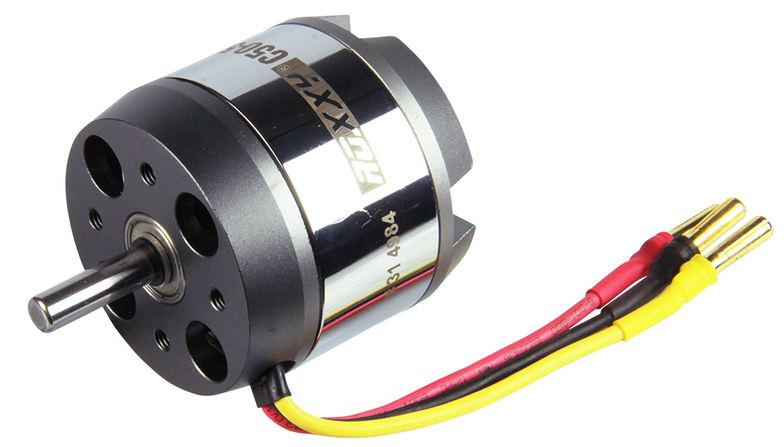
\includegraphics[width=0.6\textwidth]{images/Motor.jpg}
	\caption{Roxxy BL Outrunner C50-55-45 (100KV) \newline (Quelle: mhm-modellbau.de )}
	\label{Motor Roxxy}
\end{figure}
Drehmomentstarker, langsamdrehender Brushless-Elektromotor zum Antrieb großer Schiffs- oder U-Boot-Modelle und Segway-Roboter.

\textbf{Technische Daten:} 
\begin{itemize} 
	\item Hersteller: Multiplex 
	\item Typ: Outrunner
	\item Nenndrehzahl [kv]: 100
	\item Min. Betriebsspannung [V]: 10,0
	\item Max. Betriebsspannung [V]: 12,6
	\item Dauerstrom [A]: 16,0
	\item Gewicht [g]: 290,0
\end{itemize}
\pagebreak
\subsection{Encoder}
\begin{figure}[htb]
	\centering
	\begin{minipage}{0.38\linewidth}
		\centering
		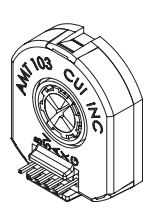
\includegraphics[scale=0.9]{images/Entcoder.jpg}
		\caption{AMT103-V  \newline (Quelle: cui.com)}
		\label{Endcoder}
	\end{minipage}
	\begin{minipage}[h]{0.6\textwidth}
		\textbf{Technische Daten:} 
		\begin{itemize} 
			\item Hersteller: CUI Inc.
			\item Modell:	AMT103-V
			\item Status der Komponente:	Aktiv
			\item Encodertyp:	Kapazitiv
			\item Ausgabetyp: Quadratur mit Index (inkremental)
			\item Impuls pro Umdrehung: Programmierbar
			\item Spannungsversorgung:	3,6 V bis 5,5 V
		\end{itemize}
	\end{minipage}
\end{figure}

\subsection{oDriver}
\begin{figure}[htb]
	\centering
	\begin{minipage}{0.38\linewidth}
		\centering
		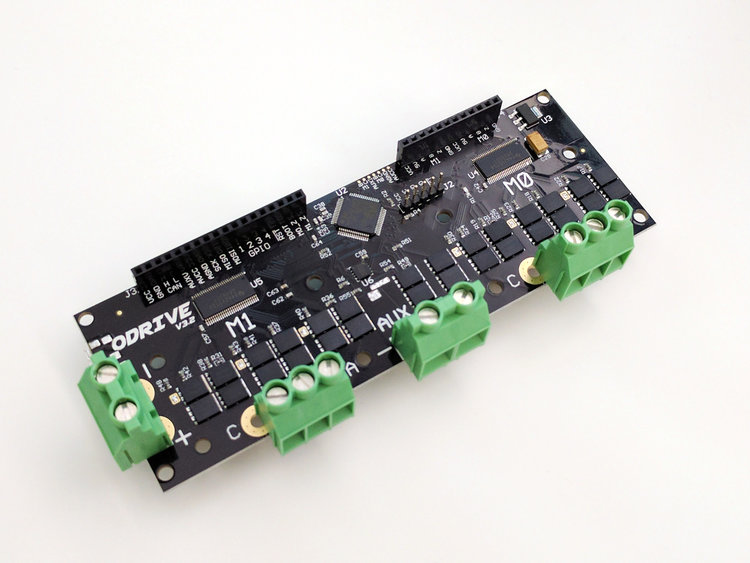
\includegraphics[scale=0.2]{images/odrive.jpeg}
		\caption{oDrive-Platine  \newline (Quelle: https://odriverobotics.com)}
		\label{odrive}
	\end{minipage}
 \begin{minipage}[h]{0.6\textwidth}
	\textbf{Technische Daten:} 
	\begin{itemize} 
		\item Zwei Motorkanäle
		\item 24V, für mehr als 100 A Spitzenstrom ausgelegt.
		\item DC-DC-Wandler für den Bremswiderstand oder Energiespeicherung.
		\item Geberrückführung für beliebig präzise Bewegungen.
	\end{itemize}
\end{minipage}
\end{figure}

\begin{itemize} 
\item Unterstützt Leistungsregeneration.
\item Optionale Verwendung einer leistungsdichten Batterie bedeutet, dass Sie erreichen können,> 1 kW Spitzenleistung mit nur einer bescheidenen Stromversorgung.
\item Open Source: Hardware , Software
\item Anschlüsse: USB Serial Port, CAN, UART, PWM
\item Schritt / Richtung - Bestehende Bewegungssteuerungen
\item Einige allgemeine digitale und analoge Stifte
\item PROTOKOLLE: Viele  Befehlsarten, 
Goto (Lageregelung mit Bahnplanung), 
Positionsbefehle, 
Geschwindigkeitsbefehl, 
Drehmomentbefehl.
\end{itemize}

\subsection{Steuerungsplatine}
\begin{figure}[!h]  % [h] bedeutet, dass das Bild genau an dieser Stelle im Text erscheint
	\centering\includegraphics[width=0.7\textwidth]{images/nucleo.jpg}
	\caption{Nucleo-F746ZG   (Quelle: playmbedded.org)}
	\label{Nucleo}
\end{figure}
\textbf{Technische Daten:}
\begin{itemize} 
	\item Mikrocontroller mit 1 MB Flash-Speicher, 320 KB SRAM, mit 216 MHz Cortex-M7-Kern STM32F746ZGT6U
	\item Adaptiver Echtzeitbeschleuniger (ART Accelerator™), der eine 0-Wartezeit-Umsetzung vom Flash-Speicher ermöglicht
	\item LCD-TFT-Controller bis XGA-Auflösung mit dediziertem Chrom-ART Accelerator™
	\item Parallele Kameraschnittstelle, 8–14 Bit, bis zu 54 MB/s
	\item Voller Zugriff auf alle GPIO mit ST Zio-Steckverbinder (Konnektivitätsunterstützung Arduino Uno v3)
	\item ST Morpho-Verlängerungsstiftleiste für den Zugriff auf alle GPIO
	\item ST-LINK/V2-1-Debugger/Programmiergerät mit SWD-Steckverbinder
	\item Bis zu 25 serielle Kommunikationsschnittstellen: USART, IrDA, I²C, SPI, LIN, CAN, USB, I²S, SDIO, HDMI-CEC, S/PDIF-Rx, Ethernet
	\item Flexibles Platinen-Netzteil
	\item USB OTG oder FS-Einheit mit micro-AB-Steckverbinder
	\item Echter Zufallszahlgenerator
	\item CRC-Kalkulationseinheit
	\item RTC mit einer Genauigkeit eines Sekundenbruchteils und Hardware-Kalender
	\item Eindeutige 96-Bit-ID
	\item Drei LEDs: Power-LED, USB-Verbindung, Benutzer-LED
	\item Benutzer- und Reset-Drucktasten
	\item Quarzoszillator, 32,768 KHz
	\item ARM mbed-fähig (mbed.org)
\end{itemize}

\subsection{Die Räder}

\begin{figure}[htb]
	\centering
	\begin{minipage}{0.49\linewidth}
		\centering
		\includegraphics[scale=0.5]{images/reifen.png}
		\caption{Räder \newline (Quelle: conrad.de)}
	\end{minipage}
	\begin{minipage}{0.4\linewidth}
		\textbf{Technische Daten:} 
		\begin{itemize} 
			\item Felgenmitnehmer - 17 mm 6-Kant
			\item Reifenbreite - 42 mm
			\item Kategorie - Kompletträder
			\item Maßstab - 1:8 
			\item Passend für Straßenmodell
			\item Reifen-Ø - 100 mm
		\end{itemize}
	\end{minipage}
\end{figure}
\pagebreak

\subsection{Die Hinderniserkenner}
\begin{figure}[htb]
	\centering
	\begin{minipage}{0.49\linewidth}
	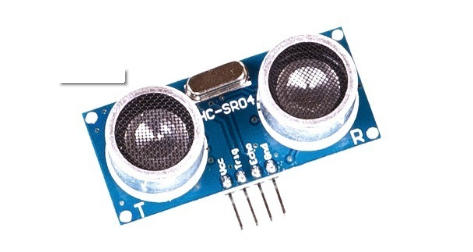
\includegraphics[scale=0.49]{images/Bild-1-1.png}
	\caption{Ultraschallsensor \newline(Quelle: conrad.de)}
\end{minipage}
\begin{minipage}{0.49\linewidth}
\textbf{Technische Daten:} 
\begin{itemize} 
			\item 	Erkennen von Umfang: 1cm-4,5 m 
			\item 	Hohe Genauigkeit: bis zu 0,2 cm
			\item 	Sensorwel: Nicht mehr als 15 Grad
			\item 	Versorgungsspannung: DC 5V
			\item Stromverbrauch: 15mA		
			\item Modus der Verbindung: VCC, trig(T), echo(R), 4. GND		
			\item Masse: 4.6 x 2 x 1,3 cm
\end{itemize}
\end{minipage}
\end{figure}

\subsection{Bewegungs- und Beschleunigungsaufnehmer}

\begin{figure}[htb]
	\centering
	\begin{minipage}{0.49\linewidth}
		\centering
		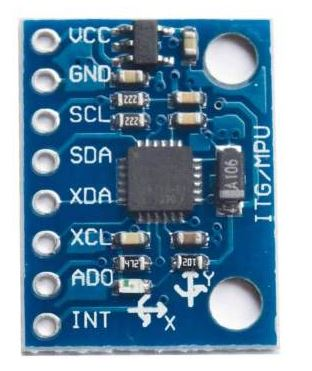
\includegraphics[scale=0.5]{images/bew.jpg}
		\caption{Bewegungs- und Beschleunigungsaufnehmer \newline (Quelle: conrad.de)}
	\end{minipage}
	\begin{minipage}{0.4\linewidth}
		\textbf{Technische Daten:} 
		\begin{itemize} 
			\item IC: MPU-6050
			\item Betriebsspannung 3V - 5V
			\item Protokoll: I2C
			\item Abmessungen: 2,0cm x 1,6 cm
		\end{itemize}
	\end{minipage}
\end{figure}
\pagebreak

\subsection{Akku}

Modellbau-Akkupack (LiPo) 11.1 V 2400 mAh 

\begin{figure}[htb]
	\centering
	\begin{minipage}{0.49\linewidth}
		\centering
		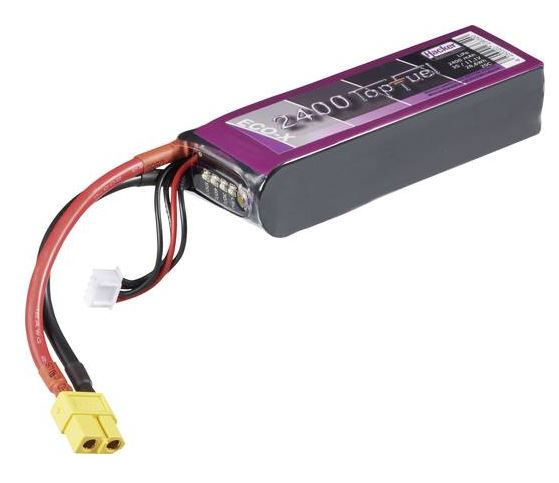
\includegraphics[scale=0.5]{images/akku.jpg}
		\caption{Akku 2400 mAh \newline (Quelle: conrad.de)}
	\end{minipage}
	\begin{minipage}{0.45\linewidth}
		\textbf{Technische Daten:} 
		\begin{itemize} 
			\item Technologie - LiPo 
		    \item Zellenanzahl - 3
			\item Spannung - 11.1 V
			\item Kapazität - 2400 mAh
			\item Belastbarkeit - 20 C
			\item Massen - 25x33x105
			\item Gewicht - 187 g
		\end{itemize}
	\end{minipage}
\end{figure}

\subsection{WLAN Router}

TP-LINK TL-WR802N WLAN Router 2.4 GHz 300 MBit/s

\begin{figure}[htb]
	\centering
	\begin{minipage}{0.49\linewidth}
		\centering
		\includegraphics[scale=0.5]{images/WLAN.jpg}
		\caption{WLAN Router \newline (Quelle: conrad.de)}
	\end{minipage}
	\begin{minipage}{0.4\linewidth}
		\textbf{Technische Daten:} 
		\begin{itemize} 
			\item WLAN-Geschwindigkeit bis 300Mbit/s
			\item WLAN-Frequenz - 2.4 GHz
			\item LAN-Übertragungsrate - 100 MBit/s
			\item Schnittstellen - LAN (10/100 MBit/s)/Micro USB
			\item Typ - TL-WR802N 
			\item Masse - 57x18x57
			\item Kompatibel zu IEEE802.11b/g/n
			\end{itemize}
	\end{minipage}
\end{figure}
\pagebreak

\subsection{Arduino - Uno}
\begin{figure}[htb]
	\centering
	\begin{minipage}{0.49\linewidth}
		\centering
		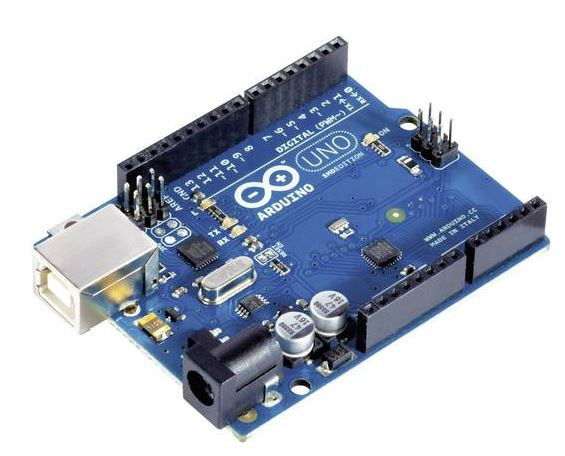
\includegraphics[scale=0.5]{images/uno.jpg}
		\caption{Arduino - Uno   \newline (Quelle: conrad.de)}
	\end{minipage}
	\begin{minipage}{0.45\linewidth}
		\textbf{Technische Daten:} 
		\begin{itemize} 
			\item Mikrocontroller - ATMega328
			\item Flash-Speicher - 32 kB
			\item Stromaufnahme - Max. 50 mA
			\item EEPROM - 1 kB
			\item Betriebsspannung - 5 V/DC
			\item Taktgeschwindigkeit - 16 MHz.
			\item SRAM - 2 kB
		\end{itemize}
	\end{minipage}
\end{figure}
\pagebreak

 

